\chapter{METODE PENELITIAN}

% Pada bagian ini, penulis akan memaparkan metodologi yang digunakan untuk
% memperdalam pemahaman mengenai aplikasi General Purpose GPU (GPGPU) dengan
% menggunakan bahasa pemrograman Julia dalam lingkup komputasi berkinerja tinggi.
% Pemilihan metode ini didasarkan pada kebutuhan untuk mendapatkan pemahaman
% komprehensif mengenai adaptasi GPU, yang secara tradisional ditujukan untuk
% pemrosesan grafis, menjadi sebuah alat yang mampu menjalankan komputasi paralel
% dan intensif. Bahasa pemrograman Julia, dikarenakan desain yang efisien dan
% modern, diidentifikasi sebagai platform yang ideal untuk memfasilitasi
% eksplorasi ini. Selanjutnya, penulis akan menjelaskan secara detail tentang
% rancangan penelitian, termasuk pemilihan dan konfigurasi perangkat keras, serta
% pendekatan dalam pemrograman yang diterapkan untuk mengoptimalkan performa
% komputasi.

Pada bagian ini, penulis akan memaparkan metodologi yang digunakan untuk
memperdalam pemahaman mengenai aplikasi General Purpose GPU (GPGPU) dengan
menggunakan bahasa pemrograman Julia dalam lingkup komputasi berkinerja tinggi.
Pemilihan metode ini didasarkan pada kebutuhan untuk mendapatkan pemahaman
komprehensif mengenai adaptasi GPU, yang secara tradisional ditujukan untuk
pemrosesan grafis, menjadi sebuah alat yang mampu menjalankan komputasi paralel
dan intensif. Bahasa pemrograman Julia, dikarenakan desain yang efisien dan
modern, diidentifikasi sebagai platform yang ideal untuk memfasilitasi
eksplorasi ini. Selanjutnya, penulis akan menjelaskan secara detail tentang
prosedur kerja, serta pemilihan dan konfigurasi perangkat keras.

\section{Bahan}

Data yang digunakan untuk melakukan operasi matriks pada penelitian ini adalah
data acak yang di-\emph{generate} oleh Julia menggunakan fungsi \cw{rand()}. Khusus pada bagian simulasi pencarian nilai eigen, digunakan bentuk matriks berdasarkan Persamaan \ref{eq:schrodinger_finite_matrix}.

\section{Alat}

Perangkat keras yang digunakan dalam penelitian ini adalah berupa komputer
dengan bentuk komputer jinjing (\emph{laptop}) dengan spesifikasi sebagai
berikut:

\begin{table}[H]
	\centering
	\caption{Spesifikasi komputer alat}
	\begin{tabular}{|M{5cm}|M{8cm}|}
		\hline
		\textbf{Komponen} & \textbf{Spesifikasi}                                   \\
		\hline
		Sistem operasi    & Manjaro Linux x86\_64 (Kernel 6.1.55-1-MANJARO)        \\
		\hline
		CPU               & Intel i7-10510U, 4.9 GHz, 4 Cores, 8 Logical Processor \\
		\hline
		GPU               & NVIDIA GeForce MX250, 2GB                              \\
		\hline
		RAM               & 20 GB                                                  \\
		\hline
		Penyimpanan       & Solid State Drive 480 GB                               \\
		\hline
	\end{tabular}
\end{table}

Kemudian, dalam menjalankan penelitian, penulis menggunakan berbagai perangkat
lunak untuk melakukan \emph{benchmarking}. Adapun perangkat-perangkat lunak
tersebut adalah:
\begin{itemize}
	\item Visual Studio Code: sebagai \emph{code editor} untuk Julia

	\item Jupyter Notebook: sebagai \emph{execution cell} untuk Julia

	\item CUDA.jl: sebagai pustaka utama untuk menjalankan paralelisasi pada
	      perangkat GPU NVIDIA

	\item Bahasa pemrograman Julia: untuk menjalankan metode fisika komputasi

	      % \item Bahasa pemgoraman Python: untuk menjalankan metode fisika komputasi
\end{itemize}

% \section{Bahan}
% Data latih dalam penelitian ini akan menggunakan data sumber distribusi $\rho$
% dari dataset acak yang memiliki rentang [-1,1] yang dibuat menggunakan program PlasmaNet
% \citep{cheng_illarramendi_bauerheim_cuenot_2021}. Dan kemudian dihitung potensial
% listrik $\phi$ menggunakan \emph{solver} Gauss-Seidel untuk plasma berbasis C++
% \citep{lubos_brieda_2019}.

% \section{Alat}
% Perangkat keras yang digunakan peneliti dalam penelitian ini adalah berupa komputer
% dengan bentuk komputer jinjing (\emph{laptop}) dengan spesifikasi sebagai
% berikut:

% \begin{table}[ht]
%   \centering
%   \caption{Spesifikasi komputer alat}
%   \begin{tabular}{|M{3cm}|M{4cm}|}
%     \hline
%     \textbf{Komponen} & \textbf{Spesifikasi}                                                            \\
%     \hline
%     Sistem operasi    & Windows 11 Home                                                                 \\
%     \hline
%     CPU               & AMD Ryzen 5 5600U with Radeon Graphics, 2.30 GHz, 6 Cores, 12 Logical Processor \\
%     \hline
%     GPU               & NVIDIA GeForce RTX 3050, 4GB                                                    \\
%     \hline
%     RAM               & 16 GB                                                                           \\
%     \hline
%     Penyimpanan       & Solid State Drive 512 GB                                                        \\
%     \hline
%   \end{tabular}
% \end{table}

% Kemudian, dalam menjalankan penelitian, penulis menggunakan berbagai perangkat lunak
% untuk membuat data, mengolah data, dan melatih data. Adapun perangkat-perangkat
% lunak tersebut adalah:
% \begin{itemize}
%   \item Visual Studio Code: sebagai pengolah kode

%   \item Google Colab Pro dengan GPU T4: untuk melatih model dengan \emph{graphic
%     processing unit} (GPU)

%   \item Bahasa pemrograman C++: untuk membangun \emph{solver} Gauss-Seidel

%   \item Bahasa pemrograman Python: untuk membangun model dan melatih model \emph{machine
%     learning}
% \end{itemize}

\section{Prosedur Kerja dan Pengambilan Data}

\begin{figure}[h]
	\centering
	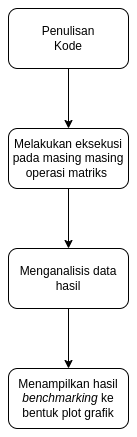
\includegraphics[width=3cm, scale=1]{schema/metode.drawio.png}
	\caption{Diagram alir penelitian}
	\label{img:methods}
\end{figure}

Secara garis besar, penelitian ini mencari waktu kecepatan eksekusi pada sistem
series (CPU) dan sistem paralel (GPU). Pada masing - masing sistem, alur
penelitian berawal dari pembuatan kode pada masing masing operasi matriks
setelah itu dilanjutkan dengan pengeksekusian kode di skenario - skenario
tertentu pada masing - masing operasi matriks, kemudian setiap hasil dari
eksekusi tersebut akan dianalisis perbedaan kecepatan eksekusi nya. Pada Gambar
\ref{img:methods} disajikan alur penelitian dengan model diagram alir atau
\emph{flowchart}.

Sistem series dan sistem paralel dituliskan dalam Bahasa Julia. Penggunaan
bahasa yang sama ini bertujuan untuk mengurangi hambatan - hambatan external
seperti hambatan karena perbedaan \emph{compiler} dari suatu bahasa pemrograman.

Proses komputasi paralel pada GPU menggunakan bantuan pustaka bernama
CUDA.jl. CUDA.jl ini merupakan pustaka untuk melakukan komputasi pada
sistem paralel GPU, khusus nya untuk Vendor GPU NVidia. Secara sederhana, cara
kerja CUDA.jl ini adalah dengan mengirimkan data array dari CPU ke \emph{vertex
	shader} di GPU, kemudian dilakukan kalkulasi yang hasilnya akan dikirimkan ke
bagian \emph{fragment shader} di GPU. Proses kalkulasi yang dijalankan di GPU disebut
dengan \textbf{kernel}. \emph{Kernel} ini pada dasarnya hanya berupa \emph{function}
Julia yang dijalankan di GPU.

\subsection{Proses Eksekusi Operasi Matriks}

Proses eksekusi diawali dengan penghasilan data sample yang mana cara
mendapatkan data sample ini sudah dijelaskan pada bagian bahan, yakni dengan
menggunakan \cw{rand()} yang merupakan fungsi \emph{random generator} dari
Julia. Setelah proses penghasilan data sudah selesai, langkah selanjutnya
adalah melakukan proses operasi matriks menggunakan CPU kemudian dilanjutkan
dengan melakukan proses operasi matriks menggunakan GPU. Proses penghasilan
data hingga proses kalkulasi menggunakan CPU dan GPU dilakukan sebanyak sepuluh
kali untuk memastikan bahwa dalam kalkulasi nya tidak terdapat hambatan
eksternal pada GPU dan CPU. Hambatan yang dimaksud antara lain seperti hambatan
kapasitas DRAM maupun VRAM yang sedang sedikit dan hambatan keterbatasan
software Jupyter dalam mengeksekusi operasi yang ada. Pada Gambar
\ref{img:methods_execution}, telah disajikan diagram alir dalam proses eksekusi
operasi matriks.

\begin{figure}[H]
	\centering
	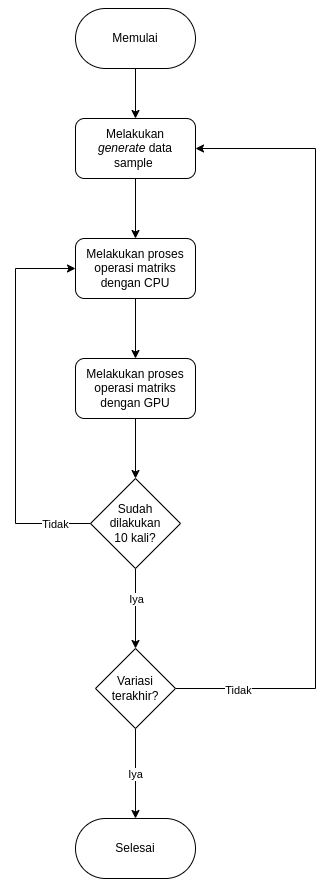
\includegraphics[width=6cm, scale=1]{schema/langkah-2.drawio.png}
	\caption{Diagram alir dalam Proses Eksekusi Setiap Metode}
	\label{img:methods_execution}
\end{figure}

Terdapat 6 operasi berbasis matriks yang dijalankan pada sistem series dan
sistem paralel sebagai berikut

\begin{enumerate}
	\item Operasi Penjumlahan Matriks
	\item Operasi Pengurangan Matriks
	\item Operasi Perkalian antara Skalar dengan Matriks
	\item Operasi Perkalian antar Matriks
	\item Inverse Matriks
	\item Pencarian Nilai Eigen
	      % \item Pencarian Nilai Eigen dari Matriks berdasarkan Persamaan  Persamaan \ref{eq:schrodinger_finite_matrix}
\end{enumerate}

\noindent
Operasi penjumlahan hingga operasi inverse matriks menggunakan data elemen bernilai acak. Namun pada operasi pencarian nilai eigen, digunakan data matriks berdasarkan Persamaan \ref{eq:schrodinger_finite_matrix}.

Pada langkah terakhir dari Gambar \ref{img:methods_execution} terdapat
pengecekan variasi percobaan. Setiap operasi matriks terdapat 7 variasi
pengukuran berdasarkan ukuran matriks nya. Berikut merupakan 7 variasi
pengukuran nya:

\begin{itemize}
	\item Variasi 1: Matriks berukuran $10 \times 10$
	\item Variasi 2: Matriks berukuran $50 \times 50$
	\item Variasi 3: Matriks berukuran $10^2 \times 10^2$
	\item Variasi 4: Matriks berukuran $500 \times 500$
	\item Variasi 5: Matriks berukuran $10^3 \times 10^3$
	\item Variasi 6: Matriks berukuran $5000 \times 5000$
	\item Variasi 7: Matriks berukuran $10^4 \times 10^4$ (Jika memungkinkan)
\end{itemize}

\noindent
Khusus untuk variasi ke-7, terkadang terdapat keterbatasan memory (RAM/VRAM) sehingga tidak memungkinkan untuk dilakukan operasi dengan besar matriks $10^4 \times 10^4$. Untuk itu, pengkaji akan menurunkan ukuran matriks hingga cukup dialokasikan ke memory, sehingga operasi bisa dijalankan.

\subsection{Analisis Data dan Penampilan Grafik}

Proses analisis data meliputi pencatatan hasil eksekusi, kemudian dilanjutkan
dengan pengumpulan semua data yang telah dicatat, kemudian yang terakhir adalah
pencarian nilai rata-rata dari sepuluh kali pengulangan. Pada Gambar
\ref{img:methods_analysist} telah disajikan diagram alir dari proses analisis
ini.

\begin{figure}[h]
	\centering
	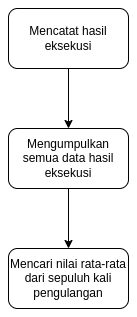
\includegraphics[width=4cm, scale=1]{schema/langkah-3.drawio.png}
	\caption{Diagram alir dalam Proses Analisis Data}
	\label{img:methods_analysist}
\end{figure}

Setelah proses analisis data selesai, langkah selanjutnya adalah penampilan
grafik berdasarkan data dari hasil analisis data. Jenis grafik yang dipilih
adalah grafik batang grup atau \emph{grouped bar chart}. Alasan dipilihnya
jenis grafik ini dikarenakan penelitian dari
\cite{hunoldBenchmarkingJuliaCommunication2020} juga menggunakan grafik batang
grup untuk menampilkan perbandingan kecepatan eksekusi Bahasa Julia dengan
Bahasa C yang mana telah dijelaskan pada Bagian Tinjauan Pustaka. Hasil grafik
akan ditampilkan dengan sumbu-x untuk perubahan variasi ukuran matriks,
sedangkan sumbu-y untuk waktu kecepatan eksekusi pada setiap operasi.

% ================================================

% \label{data_latih} Dalam konteks pemelajaran mendalam (\emph{deep learning}),
% data latih berarti pasangan data antara data masukan dan data target. Dan data hasil
% prediksi adalah data uji dan data hasil prediksi. Tahap pertama penelitian ini
% adalah pembuatan data latih. Untuk data masukan, digunakan data distribusi acak
% (sisi kanan pada Persamaan \eqref{poisson umum}) yang dibuat menggunakan program
% PlasmaNet yang dapat dikontrol skala spasialnya. Data distribusi acak memiliki
% nilai yang membentang pada rentang [-1, 1] secara kontinyu. Data ini dibuat pada
% kisi dengan resolusi kasar dengan ukuran $n_{kasar}= [n_{p}/c]$. Dengan $n_{p}$
% adalah jumlah piksel pada tiap sumbu dan $c$ adalah ukuran filter. Kemudian interpolasi
% bikubik membuat bidang random dengan ukuran struktur terkontrol pada kisi target
% \citep{cheng_illarramendi_bauerheim_cuenot_2021}, dengan $c$ adalah ukuran struktur
% minimum. Data distribusi yang diambil pada penelitian ini adalah sebanyak 20.200
% data dengan domain $100 \times 100$.

% \begin{figure}[h!]
%   \centering
%   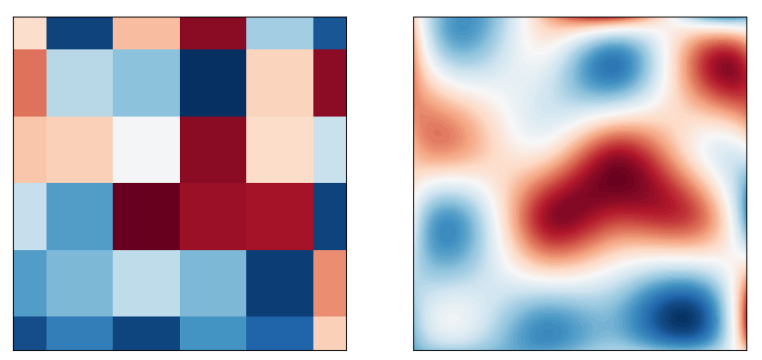
\includegraphics[width=8cm]{gambar/random.png}
%   \caption{Contoh nilai distribusi acak dalam $6 \times 6$ pada kisi kasar (kiri)
%   yang diinterpolasikan pada kisi halus $101 \times 101$ (kanan) \emph{Sumber: \citep{cheng_illarramendi_bauerheim_cuenot_2021}}}
% \end{figure}

% Tahapan pertama yang dilakukan dalam pengambilan data sekaligus dalam penelitian
% ini adalah pembuatan \emph{solver} Gauss-Seidel untuk menghasilkan pasangan
% dataset latih (\emph{training dataset}). Hal pertama yang harus diperhatikan
% dalam pembuatan program pemecah (\emph{solver}) masalah Poisson adalah domain fisis
% yang digunakan. Seperti yang telah disebutkan pada Bab \ref{tipus}, konteks pemecahan
% masalah ini adalah terletak pada koordinat silinder Gambar \ref{domain_silinder}.
% Untuk menjaga karakter kinetik model sepenuhnya, perlu dilakukan pengurangan dimensi
% sistem, membatasi domain menjadi dua dimensi ($r,z$) mengabaikan variasi azimut
% dari besaran yang terlibat (simulasi simetri aksial) \citep{f_taccogna_longo_capitelli_schneider_2005}
% dengan $r \neq 0$. Pemilihan domain ini dikarenakan ada banyak pemanfaatan yang
% dapat digunakan dalam implementasi fisis, salah satunya adalah pendorong Hall (\emph{Hall
% thruster}). Untuk itu, disesuaikanlah domain silinder ini dengan model pendorong
% Hall, adapun model domain pendorong Hall yang digunakan dalam penelitian ini adalah
% SPT-100 karena selain memiliki sejarah keberhasilan yang banyak \citep{braga_miranda_2019},
% perangkat ini juga banyak digunakan sebagai patokan atau percontohan dalam beberapa
% penelitian \citep{Shiferaw2013, f_taccogna_longo_capitelli_schneider_2005, braga_miranda_2019, boeuf_2017}.

% \begin{figure}[h!]
%   \centering
%   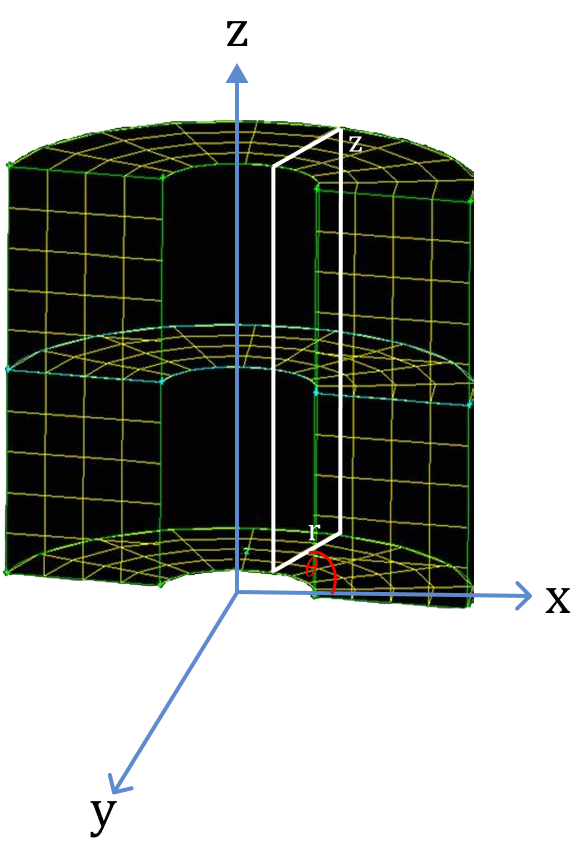
\includegraphics[width=5cm]{gambar/silinder.png}
%   \caption{Tampang lintang koordinat silinder. Penelitian ini menghitung potensial
%   listrik pada koordinat silinder dengan pendekatan simetri aksial, yaitu pada
%   sumbu $r-z$.\emph{ Sumber: \citep{Shiferaw2013} dengan penyesuaian oleh Penulis}}
%   \label{domain_silinder}
% \end{figure}

% Disadur dari \cite{braga_miranda_2019} dan \cite{f_taccogna_longo_capitelli_schneider_2005},
% spesifikasi teknis dan ukuran domain dari model SPT-100 ditampilkan dalam Tabel
% \ref{spt_100}. Domain komputasi numerik pada penelitian ini diilustrasikan dalam
% model 2 dimensi dari SPT-100 yang ditampilkan pada Gambar \ref{spt_100_2d}.

% \begin{table}[h!]
%   \centering
%   \caption{Informasi domain fisis dan teknis pendorong Hall SPT-100 }
%   \label{spt_100}
%   \begin{tabular}{ll}
%     \hline
%     \textbf{Dimensi}             & \textbf{Ukuran} \\
%     \hline
%     Panjang kanal (m)            & 0,025           \\
%     \hline
%     Lebar kanal (m)              & 0,015           \\
%     \hline
%     Panjang kanal keluar (m)     & 0,01            \\
%     \hline
%     Jari-jari silinder dalam (m) & 0,035           \\
%     \hline
%     Jari-jari silinder luar (m)  & 0,05            \\
%     \hline
%     Dorongan (N)                 & 0,08            \\
%     \hline
%   \end{tabular}
% \end{table}

% \begin{figure}[h!]
%   \centering
%   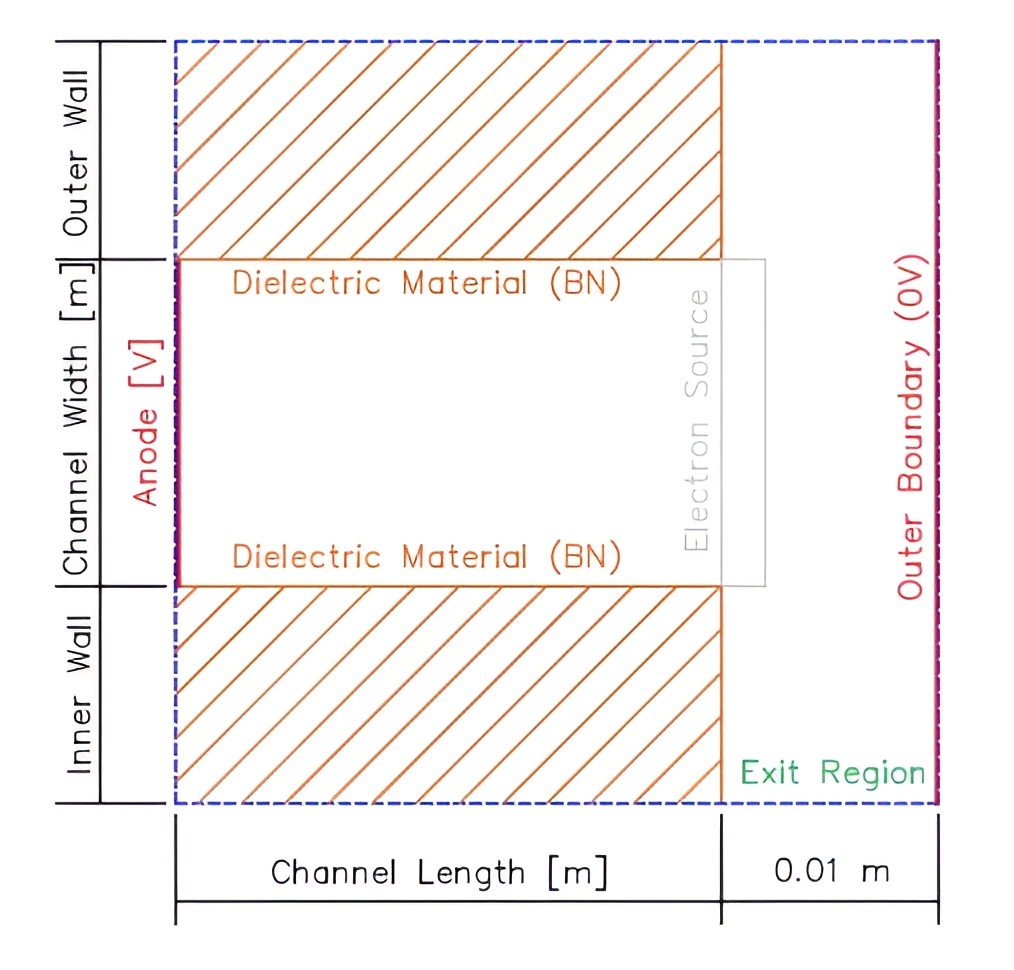
\includegraphics[width=5cm]{gambar/spt_100_2d.png}
%   \caption{Model 2 dimensi dari kanal SPT-100 sebagai domain komputasi numerik. Lebar
%   kanal dimulai dari 0,035 - 0,050 m dan panjang kanal dimulai dari 0,00 - 0,025
%   m. \emph{ Sumber: \citep{braga_miranda_2019}}}
%   \label{spt_100_2d}
% \end{figure}

% \subsubsection{Pengambilan Data Distribusi Pada Program PlasmaNet}

% Data distribusi muatan $\rho$ yang akan digunakan untuk menghitung potensial
% listrik pada pemecah Gauss-Seidel diambil menggunakan program PlasmaNet \citep{cheng_illarramendi_bauerheim_cuenot_2021}.
% Program ini menyediakan pasangan data distribusi partikel secara acak maupun
% distribusi partikel dengan pola sinusoidal dan potensial listriknya. Namun,
% pasangan data tersebut tidak dapat digunakan karena potensial listrik yang
% digunakan mengikuti syarat batas tertentu seperti pada domain komputasi yang
% disebutkan sebelumnya, sehingga hanya akan digunakan data distribusinya ($\rho$)
% saja.

% Dalam pembentukan data distribusi acak, perumusan matematis telah dijelaskan
% sebelumnya pada Subbagian \ref{data_latih}. Hal yang harus diperhatikan untuk pembuatan
% data distribusi acak ini adalah mengenai syarat awal domain serta ukuran spasial
% domain kasar dan halus. Pertama, akan ditinjau mengenai syarat awal yang digunakan
% untuk membentuk distribusi acak.

% \begin{mypythoncode}
%   [Syarat awal pembuatan data distribusi acak di PlasmaNet] xmin: 0.035 xmax: 0.050
%   nnx: 100 ymin: 0.0 ymax: 0.050 nny: 100
% \end{mypythoncode}

% Kode cuplikan Kode 1 dapat dibandingkan dengan Gambar \ref{spt_100_2d}, \texttt{xmin}
% dan \texttt{xmax} merupakan lebar kanal dan \texttt{ymin} dan \texttt{ymax} merupakan
% panjang kanal. Pada bagian ini dilakukan peniruan domain SPT-100 untuk
% distribusi muatan (Gambar \ref{ukuran spt 100}). Kemudian, \texttt{nnx} dan \texttt{nny}
% adalah jumlah piksel untuk tiap sumbu.

% \begin{figure}[h!]
%   \centering
%   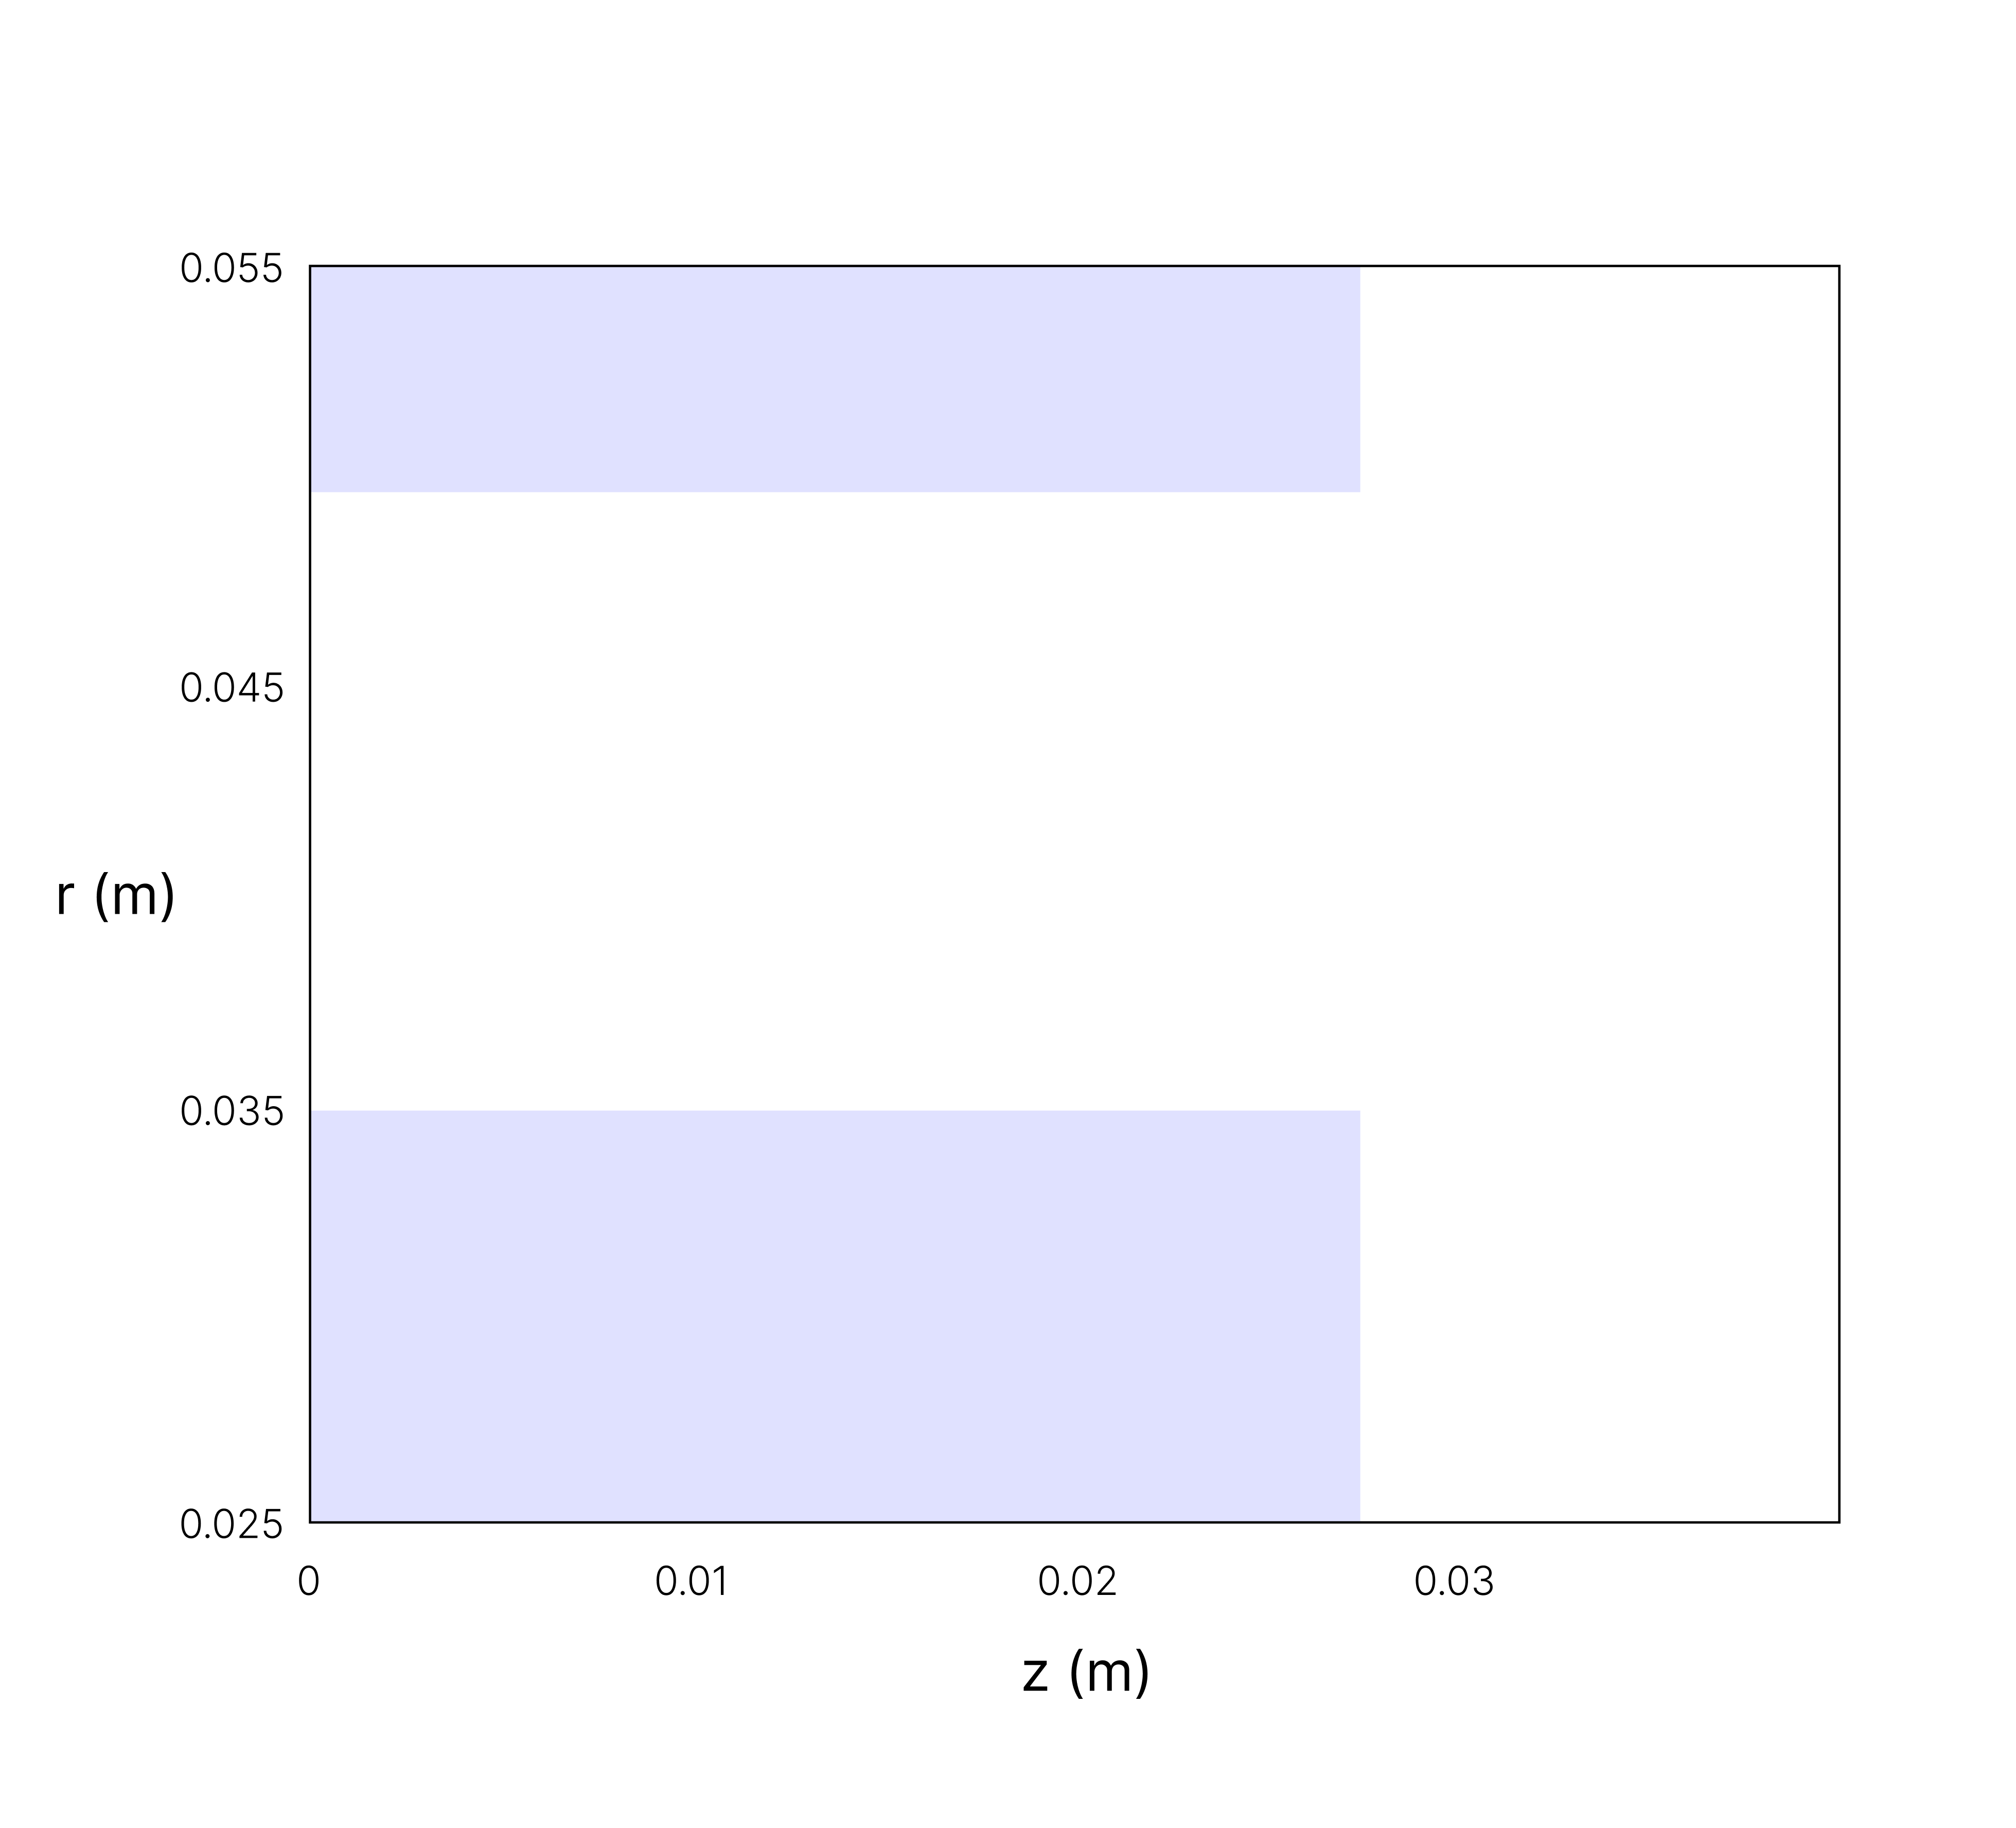
\includegraphics[width=10cm]{gambar/domain spt100 ukuran.png}
%   \caption{Ukuran kanal SPT-100. \emph{ Sumber: Penulis}}
%   \label{ukuran spt 100}
% \end{figure}

% Tahapan selanjutnya dalam pembuatan set data acak adalah memilih parameter $c$ yang
% akan menentukan ukuran struktur minimum pada ukuran domain kasar. Pada
% penelitian ini, akan digunakan domain $100 \times 100$ dan dipilih $c = 16$. Hal
% ini akan membuat domain medan acak dengan ukuran $100/8 \times 100/8 \approx 12$
% dan kemudian akan diinterpolasikan kembali ke ukuran asli $100 \times 100$.

% Setelah didapatkan kumpulan data acak, data tersebut tidak dapat langsung digunakan
% karena setelah dilakukan investigasi singkat pada data-data yang ada, nilai-nilai
% data pada set data distribusi yang dihasilkan sangat kecil (misalnya, banyak
% medan dengan nilai piksel di orde $10^{-34}$) sehingga menyebabkan kesulitan pada
% perhitungan oleh komputer. Sehingga tahapan selanjutnya adalah peningkatan (\textit{scale-up}).
% Upaya peningkatan nilai $\rho$ untuk seluruh jumlah dataset (\texttt{len(rho)}) dilakukan
% dengan cara sebagai berikut:

% \begin{mypythoncode}
%   [Kode cuplikan peningkatan nilai rho] a = len(rho) for i in range (a): rho_max
%   = np.max(rho[i]) rho_min = abs(np.min(rho[i]))

%   if rho_max > rho_min: c = 1/rho_max else: c = 1/rho_min

%   rho[i] = rho[i]*c
% \end{mypythoncode}

% Pada kode tersebut, dicari nilai ekstrim mutlak tertinggi pada tiap medan, dan
% kemudian nilai ekstrim mutlak tersebut digunakan sebagai nilai pembagi di masing-masing
% domain.

% \subsubsection{Syarat Awal dari \textit{Solver} Gauss-Seidel}

% Setelah data distribusi partikel siap, akan dilanjutkan dengan pemecahan masalah
% menggunakan metode Gauss-Seidel. Pada subbab ini dan subbab selanjutnya, akan
% dibahas mengenai syarat awal dan algoritma dari \textit{solver} Gauss-Seidel yang
% digunakan.

% Untuk membangun \textit{solver} perhitungan potensial listrik menggunakan metode
% Gauss-Seidel ini, digunakan bahasa pemrograman C++. Bahasa pemrograman C++
% dipilih pertama-tama karena bahasa ini berkali-kali lipat lebih cepat
% dibandingkan Python, walaupun Python memiliki pustaka (\textit{library}) yang
% cukup bagus dan dapat mengoptimasi kerja komputasi, semisal Numpy \citep{lubos_brieda_2019}.
% Selain itu, Python memiliki kekurangan dalam tipe variabel yang dapat memicu
% \textit{bugs}, terlebih khusus saat pembedaan variabel \textit{integer} dan \textit{floating
% point}. Dari segi pustaka, ada banyak pustaka saintifik yang diimplementasikan
% menggunakan C++ tanpa pembungkus (\textit{wrappers}) pihak ketiga.

% Syarat awal pada \textit{solver} ini didefinisikan dalam sebuah \textit{header
% file}. Dalam \textit{header file} ini berisi konstanta yang digunakan dan juga tebakan
% awal Gauss-Seidel. Pada penelitian ini digunakan satu konstanta yaitu
% $\epsilon_{0} = 8.8541878 \times 10^{-12}$ \citep{lubos_brieda_2019}. Dan untuk
% tebakan awal, digunakan nilai tebakan awal = 0 untuk seluruh piksel pada matriks
% tebakan awal.

% \subsubsection{Algoritma \textit{Solver} Gauss-Seidel}

% Pada subbagian ini akan dibahas mengenai implementasi dari Subbagian
% \ref{gauss_seidel_silinder} pada \textit{solver} Gauss-Seidel menggunakan bahasa
% pemrograman C++. Secara umum, \textit{solver} ini akan menjalankan 2 file. Yang pertama
% adalah file untuk mendefinisikan algoritma dari Gauss-Seidel sekaligus untuk menuliskan
% hasil (dalam penelitian ini file tersebut diberi nama \texttt{Potential.cpp} (Lampiran
% \ref{kode_potential_cpp})) dan file yang kedua adalah untuk memberikan syarat
% awal atau konteks besaran domain dan juga pada file ini terjadi pemanggilan
% fungsi-fungsi yang didefinisikan pada \texttt{Potential.cpp} beserta pengisian nilainya.
% Nama file ini pada penelitian ini adalah \texttt{main.cpp} (Lampiran
% \ref{kode_main_cpp}).

% Tahap paling awal pada \texttt{Potential.cpp} adalah pemanggilan \textit{header
% file} dan pustaka yang dibutuhkan. Setelah itu, dilakukan penginisialisasian menggunakan
% \textit{constructor} \texttt{Solver} untuk matriks masukan dan matriks luaran.
% Kemudian, akan didefinisikan besaran-besaran lain yang merupakan jarak domain pada
% fungsi \texttt{setextents} dan untuk jumlah iterasi maksimal dan toleransi ralat
% diatur pada fungsi \texttt{setParam}.

% Setelah semua kondisi diatur, masuk pada perhitungan iterasi pada fungsi \texttt{writeSolveGS}.
% Di sini, argumen yang digunakan adalah \texttt{filename}, \texttt{reshape\_\texttt{\-}rows},
% \texttt{reshape\_cols}, yang nilai argumennya semuanya terletak pada \texttt{main.cpp}.
% Berikut adalah \textit{pseudocode} dari algoritma implementasi perhitungan Gauss-Seidel:
% \begin{lstlisting}[breaklines=true, breakatwhitespace=true]
% DEFINISIKAN variabel: idz, idr, idz2 (idz pangkat dua), idr2 (idr pangkat dua), crz
% SET L2 ke 0
% SET converged ke False

% FOR iterasi < nilai iterasi maksimal:
%     iterasi ditambah 1
%     FOR i < jumlah baris keseluruhan data:
%         i ditambah 1
%         FOR j < jumlah kolom:
%             j ditambah 1
%             IF i = 0 ATAU i kelipatan 100: #syarat batas paling atas
%                 CONTINUE
%             ELSE IF i modulo 100 = 99: #syarat batas paling bawah
%                 phi(i,j) = phi(i-1, j)
%             ELSE IF j = 0: #syarat batas paling kiri
%                 CONTINUE
%             ELSE IF j = 99: #syarat batas paling kanan
%                 CONTINUE
%             ELSE: #selain di syarat batas (interiornya)
%                 hitung crj
%                 hitung phi baru menggunakan rho dari file yang ada
%                 lanjutkan dengan SOR

%     IF iterasi kelipatan 100:
%         hitung L2 antara 2 iterasi

%         IF L2 < nilai toleransi
%             perhitungan konvergen atau converged = True
%             BREAK

%     IF tidak konvergen:
%         tampilkan teks: "Gauss seidel standar gagal konvergen, L2=", masukkan nilai L2

%     #penulisan hasil phi pada file csv
%     FOR i < jumlah baris keseluruhan data:
%         i ditambah 1
%         FOR j < jumlah kolom:
%             j ditambah 1
%             IF j pada indeks kolom terakhir:
%                 tulis phi(i,j) diikuti pindah baris
%             ELSE
%                 tulis phi(i,j) diikuti tanda koma (,)
% \end{lstlisting}

% Variabel-variabel yang didefinisikan di awal merupakan variabel yang akan
% digunakan pada perhitungan interior domain, yang detail perhitungannya dapat dilihat
% pada kode sumber. Untuk syarat batas pada atas, kiri, dan kanan, diimplementasikan
% syarat batas Dirichlet nol, sedangkan pada batas paling bawah diterapkan syarat
% batas Neumann. Pada perhitungan Gauss-Seidel di interior menggunakan implementasi
% penyelesaian persamaan Poisson menggunakanm metode Gauss-Seidel seperti pada Subbagian
% \ref{gauss_seidel_silinder} dan parameter SOR 1,4 untuk mempercepat konvergensi seperti
% pada \cite{lubos_brieda_2019}.

% Setiap 100 iterasi, dihitung nilai metrik L2 untuk menentukan nilai ralatnya. Nilai
% L2 ini merupakan nilai rerata ralat dari seluruh piksel iterasi tersebut dengan iterasi
% sebelumnya. Apabila nilai setelah iterasi ke-100 nilai L2 sudah di bawah nilai
% toleransi, maka iterasi pada medan tersebut dihentikan. Namun apabila belum,iterasi
% dilanjutkan pada iterasi kelipatan 100 lainnya dan diperiksa lagi apakah sudah
% di bawah nilai toleransi. Apabila nilai L2 pada medan tersebut belum sampai di bawah
% nilai toleransi sampai pada jumlah iterasi maksimal, maka iterasi pada medan
% tersebut dianggap gagal dan program akan mengeluarkan pesan galat "Gauss seidel standar
% gagal konvergen, L2=" diikuti dengan nilai L2 terakhir.

% Untuk memanggil fungsi-fungsi yang ada pada program Lampiran
% \ref{kode_potential_cpp}, digunakan program lain, yaitu program pada Lampiran
% \ref{kode_main_cpp}. Dalam Lampiran \ref{kode_main_cpp} ditampilkan contoh kasus
% saat program menghitung 2.000 data. Variabel \texttt{nz} adalah jumlah baris keseluruhan
% data, sehingga nilainya $2.000 \times 100 = 200.000$, dan variabel \texttt{nr}
% adalah jumlah kolom domain, yaitu 100.

% Variabel \texttt{totalData} merupakan jumlah seluruh piksel yang dilibatkan dalam
% perhitungan ini. File \textit{comma separated value} (CSV) dari data distribusi yang
% digunakan dipanggil pada variabel \texttt{rho} yang kemudian diubah bentuknya
% menjadi $nz \times nr$. Untuk parameter domain SPT-100 (Tabel \ref{spt_100}) didefinisikan
% pada pemanggilan fungsi \texttt{setextents}. Jumlah iterasi maksimal yang digunakan
% pada perhitungan ini sebesar 100.000 dan nilai toleransi yang diizinkan adalah 0,01.
% Kedua parameter tersebut didefinisikan pada fungsi \texttt{setParam}. Tidak ada referensi
% baku mengenai nilai maksimal iterasi dan nilai ralat yang digunakan. Pada
% \cite{lubos_brieda_2019}, untuk ukuran domain $21 \times 21 \times 21$ sebanyak 1
% data, digunakan nilai iterasi maksimal 5000 dan nilai toleransi 0. Berdasarkan
% acuan ini, dicoba nilai iterasi maksimal dan nilai toleransi ralat yang wajar,
% dapat diandalkan, serta realtif cepat untuk domain 100 $\times$ 100 dengan 2.000
% data (digunakan jumlah 2.000 data dalam sekali perhitungan untuk mencegah agar
% jangan sampai terjadi kerusakan pada perangkat keras karena durasi \textit{runtime}
% yang terlalu lama dan penggunaan memori yang terlalu besar), maka digunakan jumlah
% iterasi maksimal sebanyak 100.000 dan toleransi ralat sebesar 0,01.

% Selain data latih, untuk melatih model yang ada, dibutuhkan data validasi (\emph{validation
% data}) untuk melihat peforma dari model tanpa bias dari data latih \citep{jason_brownlee_2017}.
% Dalam penelitian ini, data validasi diambil sebanyak 25\% dari total data latih.

% \subsection{Pengambilan Data Uji}
% Setelah model didapatkan untuk dilatih, kemudian model diuji dengan data lain
% yang tidak pernah dilihat sebelumnya oleh model. Data tersebut sebagian merupakan
% kumpulan data dengan distribusi acak dan sebagian merupakan data dengan distribusi
% partikel mengikuti aturan Gaussian (Persamaan \eqref{gaussian}):

% \begin{equation}
%   \label{gaussian}f(x,y) = A \enspace exp \left(-\left(\frac{(x-x_{0})^{2}}{2
%   \sigma^{2}_{X}}+ \frac{(y-y_{0})^{2}}{2 \sigma^{2}_{Y}}\right)\right)
% \end{equation}

% Dengan $A$ adalah amplitudo, $x_{0}$ dan $y_{0}$ merupakan koordinat titik pusat,
% dan $\sigma_{x}$, $\sigma_{y}$ merupakan standar deviasi pada sumbu $x$ dan $y$.

% \subsection{Pemrosesan data}
% Salah satu keuntungan terbesar penggunaan jaringan saraf buatan adalah, tidak perlu
% dilakukan \emph{feature engineering}. Lapisan tersembunyi (\emph{hidden layer})
% yang akan mempelajar fitur-fitur dari data yang diberikan \citep{denny2015}.
% Sehingga tidak diperlukan pemrosesan data yang membutuhkan usaha besar.

% Pemrosesan data yang dilakukan adalah pengubahan dimensi bentuk dan normalisasi.
% Perubahan bentuk dalam hal ini adalah pengubahan data-data menjadi masing-masing
% bentuk matriks persegi dalam satu kolom. Kemudian dilakukan normalisasi untuk
% mentransformasi fitur menjadi skala yang mirip, sehingga meningkatkan peforma dan
% stabilitas pelatihan model \citep{google_2022}. Normalisasi yang dilakukan adalah
% penskalaan (\emph{scaling}). Penskalaan berarti mengubah nilai titik data dari rentang
% aslinya ke rentang standar (biasanya 0 sampai 1 atau -1 sampai 1).

% \subsection{Pendefinisian arsitektur}

% Pendefinisian arsitektur dilakukan sesuai dengan bentuk data yang masuk dan bentuk
% data luaran yang dikehendaki. Penambahan regulator, \emph{pooling layer}, dan \emph{padding}
% juga dilakukan di sini. Tidak ada patokan yang baku mengenai bentuk arsitektur dan
% \emph{hyperparameter} yang akan digunakan. Penentuannya akan dilakukan dengan metode
% \emph{trial and error}.

% \subsection{Pelatihan model}
% Model atau arsitektur yang sudah ada kemudian dilatih atau di-\emph{fitting} dengan
% data latih yang disediakan dan divalidasi dengan data validasi yang terpisah dari
% data latih. Pada proses pelatihan ini menggunakan fungsi ralat MSE \ref{mse}, dengan
% \emph{batch size} 32, 200 \emph{epoch}. Kemudian dengan menggunakan pengoptimasi
% ADAM \citep{kingma2017adam} dengan laju pemelajaran awal (\emph{inital learning
% rate}) = 0.001 dan diterapkan penjadwalan laju pemelajaran dengan langkah peluruhan
% (\emph{decay steps}) = 10000 dan laju peluruhan (\emph{decay rate}) = 0.9.

% Sembari dilatih, semua model dari tiap \emph{epoch} disimpan dalam bentuk file h5
% dan kemudian dipilih model yang paling baik dengan cara melihat kurva pemelajaran
% yang muncul setelah model terlatih seutuhnya. Kriteria model yang paling baik
% adalah model dengan \emph{validation loss} paling rendah dan berada di bawah atau
% sama atau hampir sama dari \emph{training validatrion} (\emph{goodfit}).

% \subsection{Evaluasi dan pengujian}
% Masuk ke tahap evaluasi dan pengujian, pertama akan dimuat data uji yang sudah
% dibuat sebelumnya. Kemudian, muat model \emph{epoch} ke-100, \emph{epoch} ke-200,
% dan \emph{epoch} dengan model paling baik. Kemudian lakukan prediksi dengan data
% distribusi $\rho_{uji}$ untuk tiap model.

% Selanjutnya, akan dibandingkan $\phi_{pred}$ yang merupakan hasil prediksi model
% dan $\phi_{uji}$. Sebelum dilakukan pembandingan, data $\phi_{uji}$ dilakukan normalisasi
% terlebih dahulu. Uji yang pertama adalah uji visual pada matriks yang diuji. Di sini
% akan dilihat secara visual seberapa mirip antara $\phi_{uji}$ dan $\phi_{pred}$.

% Selanjutnya akan dipilih beberapa piksel secara acak untuk diketahui nilainya,
% baik pada $\phi_{uji}$ maupun $\phi_{pred}$. Data piksel tersebut kemudian dibandingkan
% dengan cara dihitung MSE dan MAPE-nya.

% Uji selanjutnya adalah pengujian menggunakan MAPE. Akan dipilih nilai-nilai yang
% jauh dari nol. Kemudian dihitung MAPE dari nilai tersebut. Dari pengujian
% tersebut ditentukan nilai MAPE tertinggi, MAPE terendah, dan rata-rata dari
% keseluruhan MAPE.

% =========================

% Please add the following required packages to your document preamble:
% \usepackage{lscape}
% \usepackage{longtable}

% Note: It may be necessary to compile the document several times to get a multi-page table to line up properly

% \begin{landscape}
%   \subsection{Rencana Kegiatan Penelitian}
%   \begin{longtable}[c]{|l|l|l|l|l|l|l|l|l|l|l|l|}
%     \caption{Tabel Rencana Kegiatan November 2023 -- Mei 2024}
%     \label{table:plan}                                                                                                                                                                                 \\
%     \hline
%     No.                                                                                                                   & Kegiatan & November  & Desember & Januari & Februari & Maret & April & Mei \\ \hline
%     \endfirsthead
%     %
%     \multicolumn{12}{c}%
%     {{\bfseries Table \thetable\ continued from previous page}}                                                                                                                                        \\
%     \hline
%     No.                                                                                                                   & Kegiatan & Novermber & Desember & Januari & Februari & Maret & April & Mei \\ \hline
%     \endhead
%     %
%     1                                                                                                                     &
%     \begin{tabular}[c]{@{}l@{}}Eksplorasi Bahasa Julia dan pustaka nya\end{tabular}                                       &
%     \checkmark                                                                                                            &
%     \checkmark                                                                                                            &
%                                                                                                                           &
%                                                                                                                           &
%                                                                                                                           &
%                                                                                                                           &
%     \\ \hline
%     %
%     2                                                                                                                     &
%     \begin{tabular}[c]{@{}l@{}}Penulisan Proposal\end{tabular}                                                            &
%     \checkmark                                                                                                            &
%     \checkmark                                                                                                            &
%     \checkmark                                                                                                            &
%     \checkmark                                                                                                            &
%                                                                                                                           &
%                                                                                                                           &
%     \\ \hline
%     %
%     3                                                                                                                     &
%     \begin{tabular}[c]{@{}l@{}}Penulisan Kode dan Pengeksekusian \\ Operasi Penjumlahan Matriks\end{tabular}              &
%                                                                                                                           &
%                                                                                                                           &
%                                                                                                                           &
%     \checkmark                                                                                                            &
%                                                                                                                           &
%                                                                                                                           &
%     \\ \hline
%     %
%     4                                                                                                                     &
%     \begin{tabular}[c]{@{}l@{}}Penulisan Kode dan Pengeksekusian \\ Operasi Pengurangan Matriks\end{tabular}              &
%                                                                                                                           &
%                                                                                                                           &
%                                                                                                                           &
%     \checkmark                                                                                                            &
%                                                                                                                           &
%                                                                                                                           &
%     \\ \hline
%     %
%     5                                                                                                                     &
%     \begin{tabular}[c]{@{}l@{}}Penulisan Kode dan Pengeksekusian \\ Operasi Perkalian Matriks dengan Skalar\end{tabular}  &
%                                                                                                                           &
%                                                                                                                           &
%                                                                                                                           &
%     \checkmark                                                                                                            &
%     \checkmark                                                                                                            &
%                                                                                                                           &
%     \\ \hline
%     %
%     6                                                                                                                     &
%     \begin{tabular}[c]{@{}l@{}}Penulisan Kode dan Pengeksekusian \\ Operasi Perkalian Matriks dengan Matriks\end{tabular} &
%                                                                                                                           &
%                                                                                                                           &
%                                                                                                                           &
%     \checkmark                                                                                                            &
%     \checkmark                                                                                                            &
%                                                                                                                           &
%     \\ \hline
%     %
%     7                                                                                                                     &
%     \begin{tabular}[c]{@{}l@{}}Penulisan Kode dan Pengeksekusian \\ Operasi Inverse Matriks\end{tabular}                  &
%                                                                                                                           &
%                                                                                                                           &
%                                                                                                                           &
%                                                                                                                           &
%     \checkmark                                                                                                            &
%                                                                                                                           &
%     \\ \hline
%     %
%     8                                                                                                                     &
%     \begin{tabular}[c]{@{}l@{}}Penulisan Kode dan Pengeksekusian \\ Nilai Eigen \end{tabular}                             &
%                                                                                                                           &
%                                                                                                                           &
%                                                                                                                           &
%                                                                                                                           &
%     \checkmark                                                                                                            &
%                                                                                                                           &
%     \\ \hline
%     %
%     9                                                                                                                     &
%     \begin{tabular}[c]{@{}l@{}} Pengumpulan dan Analisis Semua data \end{tabular}                                         &
%                                                                                                                           &
%                                                                                                                           &
%                                                                                                                           &
%                                                                                                                           &
%     \checkmark                                                                                                            &
%     \checkmark                                                                                                            &
%     \\ \hline
%     10                                                                                                                    &
%     \begin{tabular}[c]{@{}l@{}} Penulisan Hasil dan Pembahasan \end{tabular}                                              &
%                                                                                                                           &
%                                                                                                                           &
%                                                                                                                           &
%                                                                                                                           &
%     \checkmark                                                                                                            &
%     \checkmark                                                                                                            &
%     \checkmark                                                                                                                                                                                         \\ \hline
%   \end{longtable}
% \end{landscape}
